\chapter{Data Analysis}
%A detailed explanation of the attributes of the data. discrete/continos, nominal/ordinal/interval/radio). Data issues like missing values, corrupted data. The basic summary statistics of the attributes.

\section{Introduction}
In this chapter a detailed explanation of the attributes will be given. It will be shown how the attributes are somewhat correlated and the real dimensionality of the data will be found using Principal Component Analysis (PCA). 

\section{Basic Statistic Properties}
By means of the ACCENT\footnote{Apprehension, clarity, consistency, efficiency, necessity and truthfulness} principles some interesting figures have been made in Matlab to illustrate some properties of the data. Some summary statistics have also been omitted as them not contributing any further information for this data set. An example of this is computing the mean and standard deviation(std). Instead the std has been computed from standardized data, for 2000 randomly drawn samples, and plotted in Figure~\ref{fig:1b}. 
 
\begin{figure}[H]
\begin{minipage}[t]{.49\linewidth}
\centering
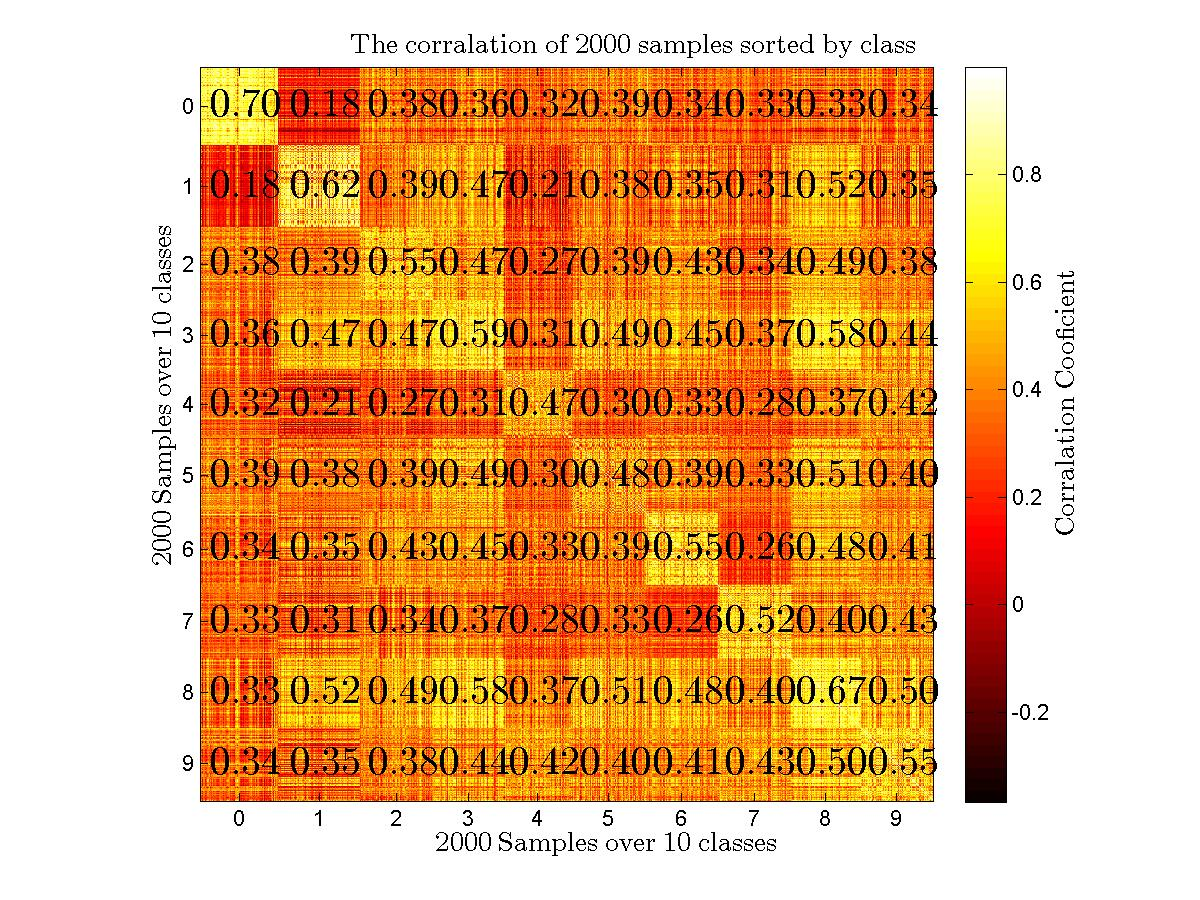
\includegraphics[width=\linewidth]{corr_explained}
\subcaption{The correlation of 2000 randomly drawn samples sorted by class. The mean of each class-by-class square have its mean value printed ontop. \label{fig:1a}}
\end{minipage}%
\hfill%
\begin{minipage}[t]{.49\linewidth}
\centering
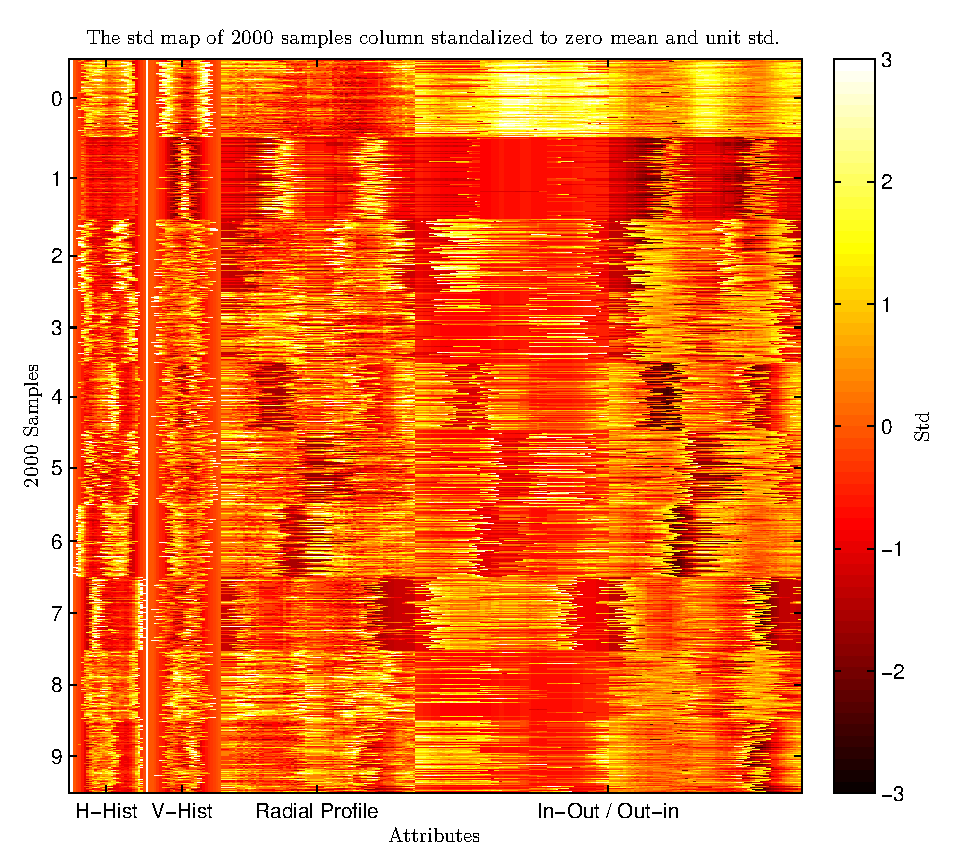
\includegraphics[width=\linewidth]{std_explained}
\subcaption{The std of all attributes from the same 2000 samples in Figure~\ref{fig:1a}. \label{fig:1b}}
\end{minipage}
\caption{Conclusion: Classes are clearly correlated and it should be possible to apply classification routines to separate the classes. }
\end{figure}

From Figure~\ref{fig:1b} some properties can be seen. One example would be the class of zeros in-out profile are significant higher than the average and classes of ones have its horizontal histogram below average near the middle and higher in the middle. Keeping this information in mind and returning to Figure~\ref{fig:image_examples} this becomes truth when looking at the features. The ten zeros shown earlier have a medium respond for the in-out profile while the five other classes have almost zeros. It also makes sense that ones have high response at the middle because of ones being vertical lines and nothing around them.

\subsection{Correlation}
In Figure~\ref{fig:1a} the correlation of samples have been computed and sorted by classes. Furthermore the mean value for each class by class square box have been computed and plotted on top for truthfulness when colours fails. It can been seen that classes has some correlation with the other classes, but important is that each class is mostly correlated with its own class. The fact that some classes do not correlate a lot to itself is likely based on the fact that people tend to write this digit in many different ways (i.e. the digit 4).

\begin{figure}[H]
\centering
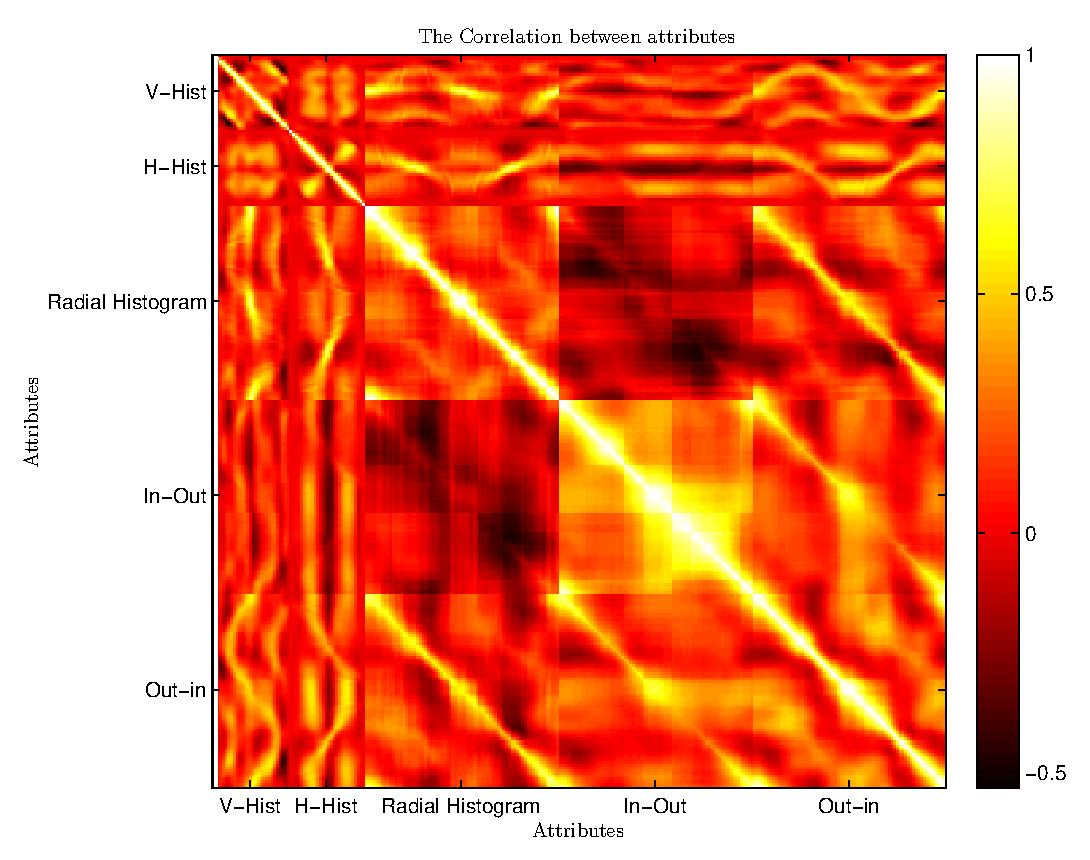
\includegraphics[width=0.49\linewidth]{att_corr_explained}
\caption{The correlation of attributes. Conclusion: Highly correlated and dimension can be reduced.\label{fig:att_corr_explained}}
\end{figure}

It can also be very interesting to look at correlation between attributes, as shown in Figure~\ref{fig:att_corr_explained}. It's seen that the attributes are highly correlated in parts of the plot and it also make sense when looking back on the feature generation. The histograms correlate and some kind of symmetry is shown in the figure. This could very well be explained by the fact that a lot of the digits actually also have symmetric parts. Instead of speculating in such relationships, a PCA will be used to find the real dimension of the data.  



\inputtex{pca}